We have chosen to make some changes in the User Interface available in the front-end in order to take advantage of the features provided by \textit{\gls{ckan}}. In what concerns the pages alluding to datasets and resources, as well as those of groups and organisations, we consider that the information is already provided in an intuitive way and, in our opinion, does not need any changes. Nevertheless, we consider that the homepage could suffer some changes, and, as such, we opted to work on it and obtained the result shown in the figure \ref{tab:homepage}.

\begin{figure}[!h]
    \centering
    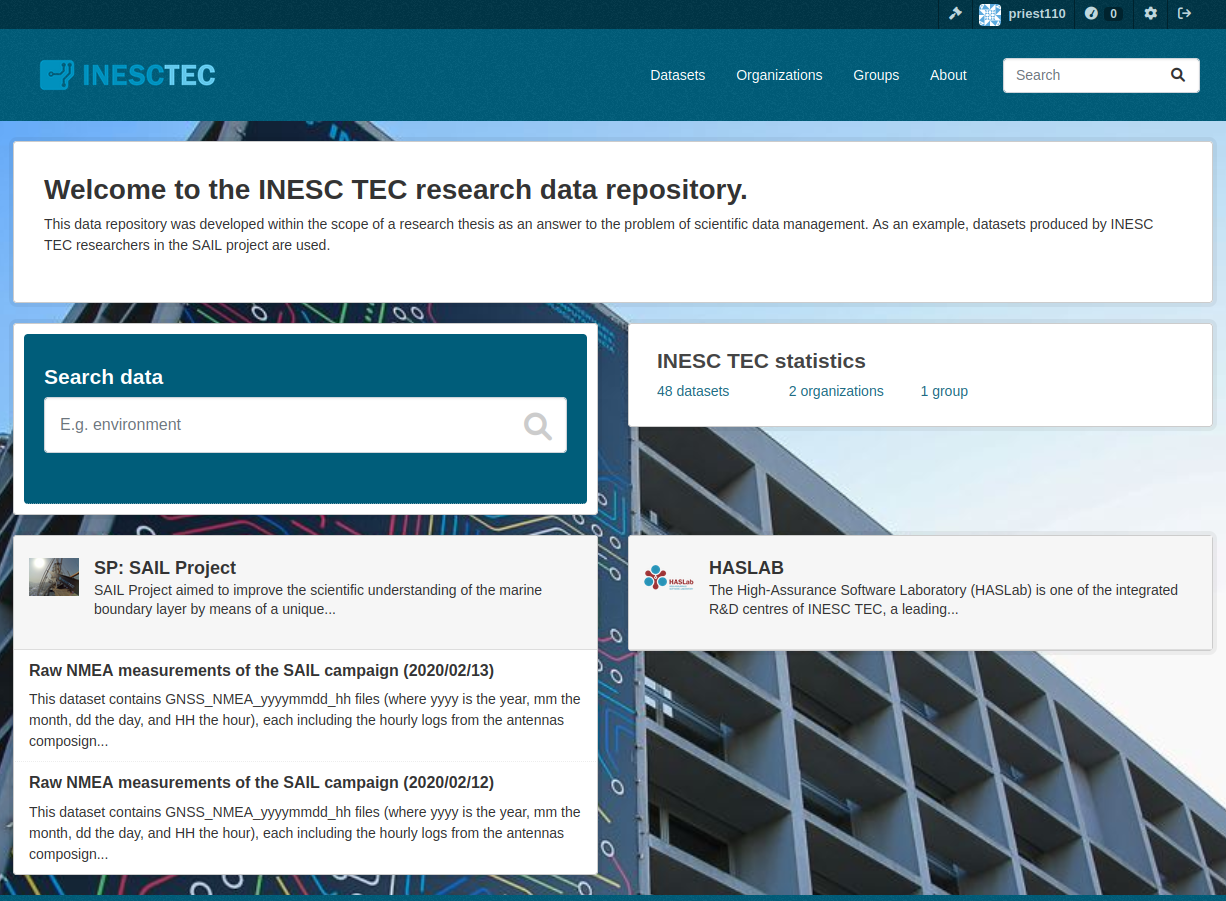
\includegraphics[width=1\textwidth]{img/solution/UI.png}
    \caption{\label{tab:homepage} Homepage}
\end{figure}

Thus, we have improved the initial aesthetics of the main page (which ends up being the first thing that users will see in the system) and we have customised it to fit in with the institution that uses its services. Furthermore, as the primary reason for the change, we have been able to transmit more useful information, as previously only the welcome statement, the search engine, and the statistics were considered, and now it is also possible to access two additional components:

\begin{itemize}
    \item Latest group in the system, in this case associated with \gls{sail} Project, and its two latest resources;
    \item The most recent organization in the system, which is HASLab, and which in turn does not yet have any associated resources.
\end{itemize}